\chapter{Concluzii și rezultate}

\section{Obiectivele atinse}

Aplicația mobilă pentru recunoașterea și interpretarea informațiilor nutriționale a reușit să îndeplinească cu succes obiectivele propuse inițial. Prin implementarea unei soluții complete care combină tehnologiile OCR cu inteligența artificială, s-a creat un instrument eficient pentru automatizarea procesului de analiză nutrițională.

Principalele obiective realizate includ:

\textbf{Automatizarea extragerii datelor nutriționale:} Sistemul OCR și AI implementat folosind o combinație dintre Tesseract și Google Gemini API reușește să extragă cu precizie informațiile nutriționale din imaginile etichetelor alimentare. Testările efectuate pe diverse tipuri de etichete au demonstrat rezultate pozitive pentru informațiile nutriționale standard și pentru listele de ingrediente complexe.

\textbf{Interpretarea inteligentă a ingredientelor:} Integrarea cu Google Gemini API a permis transformarea listelor complexe de ingrediente în explicații ușor de înțeles pentru utilizatori. Sistemul AI identifică cu succes componentele benefice și dăunătoare, oferind context științific pentru denumirile tehnice și calculând un scor de procesare bazat pe natura ingredientelor.

\textbf{Experiența utilizatorului optimizată:} Aplicația mobilă dezvoltată în React Native oferă o interfață intuitivă și responsivă. Procesul de adăugare a unui aliment se realizează rapid, iar rezultatele analizei sunt disponibile în timp real prin sistemul de task-uri în background.

\textbf{Arhitectura scalabilă:} Utilizarea Docker Compose și a unei arhitecturi bazate pe microservicii permite scalarea orizontală a sistemului și integrarea cu aplicații externe prin API-ul RESTful dezvoltat.

\begin{figure}[h!]
    \centering
    \begin{minipage}{0.45\textwidth}
        \centering
        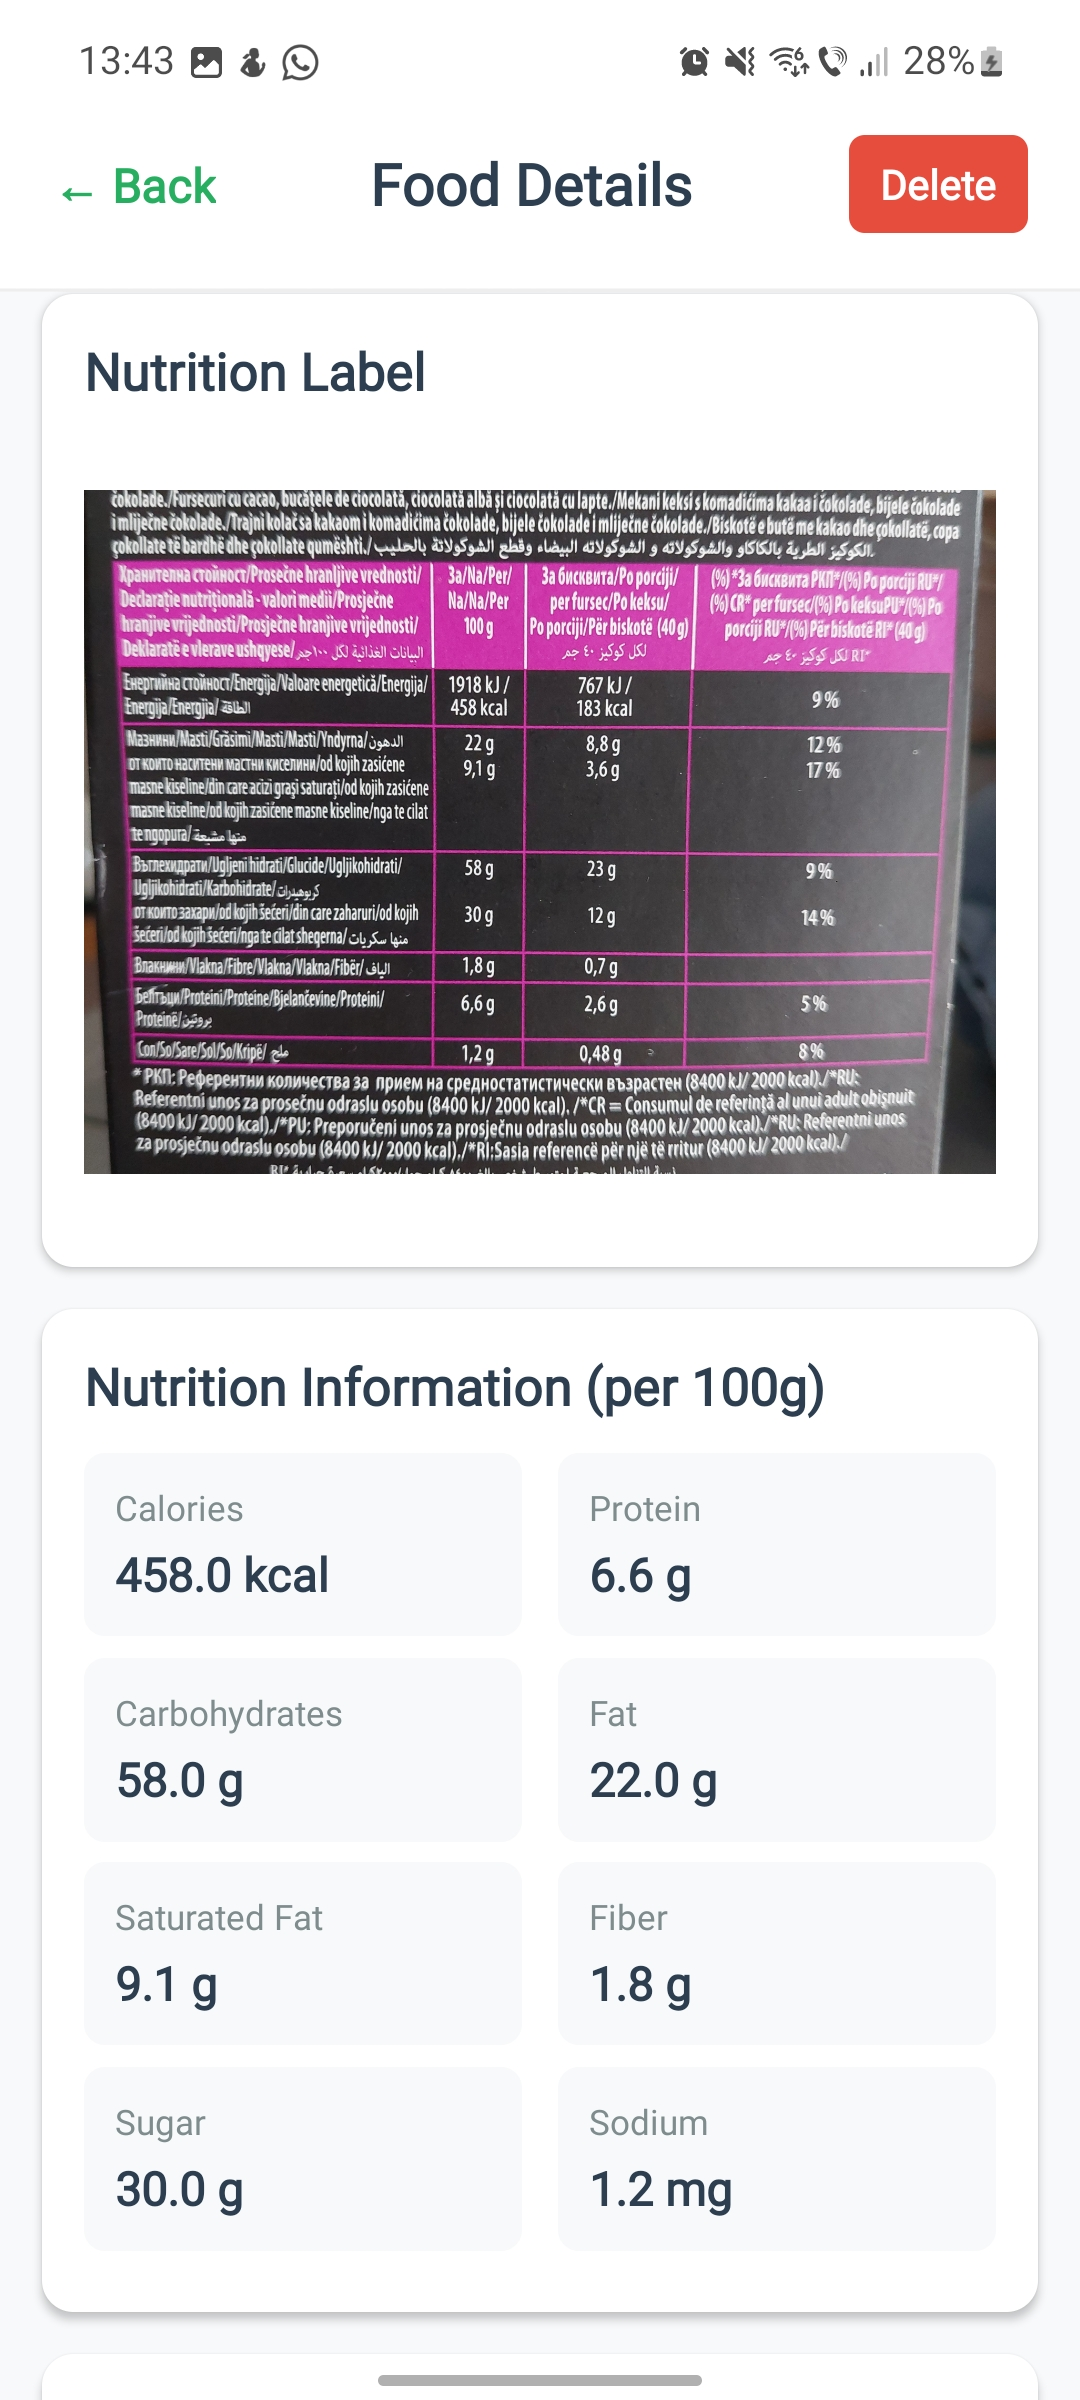
\includegraphics[width=0.9\textwidth]{images/Nutritional_info.jpg}
        \caption{Captură de ecran cu informațiile nutriționale extrase dintr-o etichetă alimentară.}
        \label{fig:nutritional-info-conclusions}
    \end{minipage}
    \hfill
    \begin{minipage}{0.45\textwidth}
        \centering
        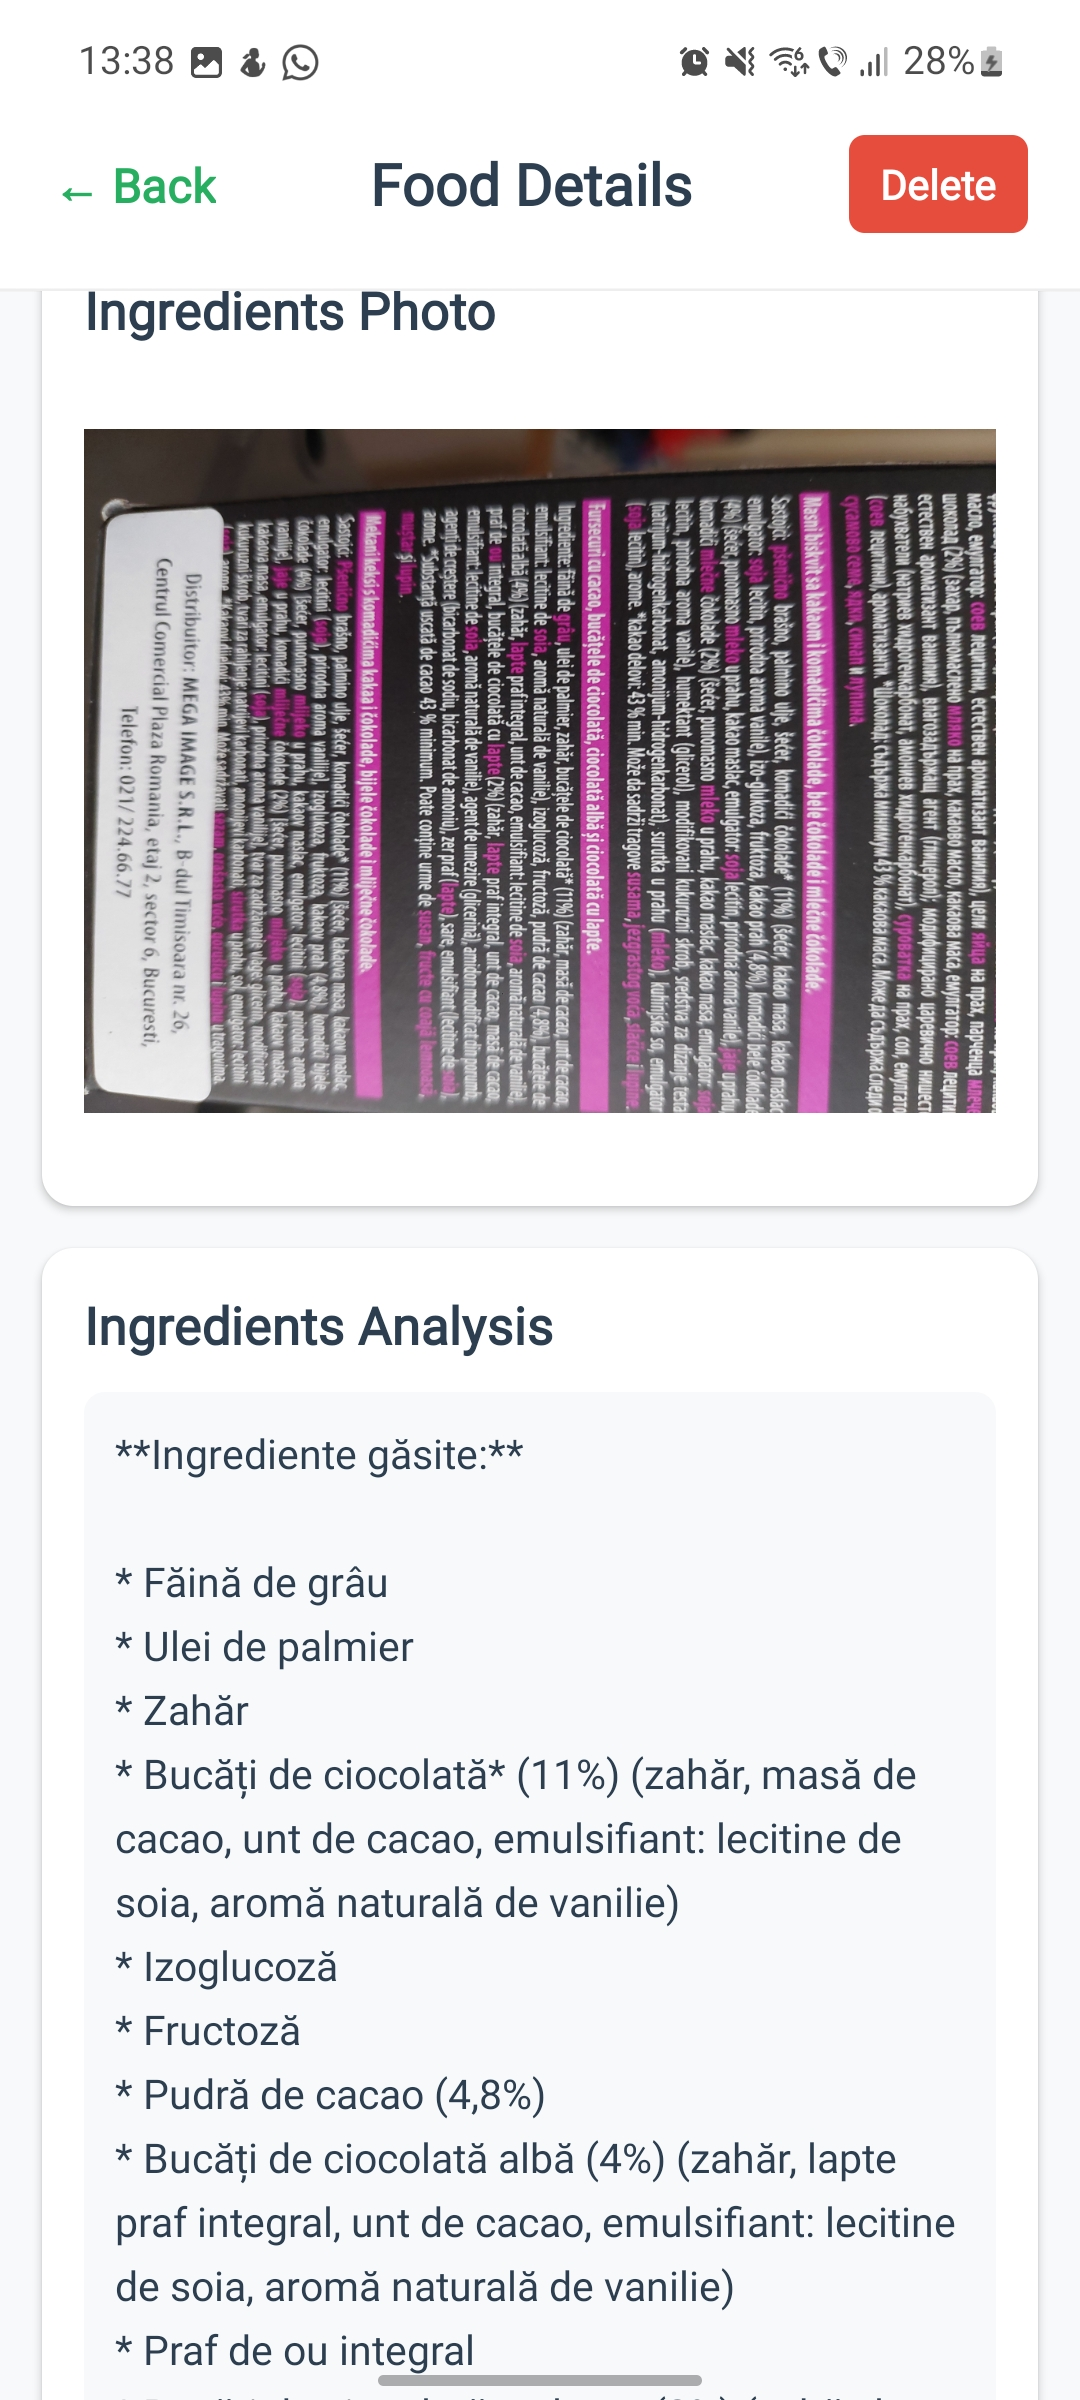
\includegraphics[width=0.9\textwidth]{images/Ingredients_info_1.jpg}
        \caption{Captură de ecran cu informațiile despre ingrediente extrase dintr-o poză cu ingrediente.}
        \label{fig:ingredients-info-1-conclusions}
    \end{minipage}
\end{figure}

\section{Rezultate obținute}

\subsection{Funcționalitatea sistemului OCR}

Sistemul OCR implementat folosind Tesseract demonstrează capacități solide în extragerea informațiilor nutriționale din imaginile etichetelor alimentare. Testările pe diverse tipuri de etichete au evidențiat că sistemul funcționează cel mai bine pe etichete cu fond alb și text negru, oferind rezultate consistente pentru valorile numerice standard precum caloriile, proteinele, grăsimile și carbohidrații.

Provocările principale identificate includ procesarea etichetelor cu fonduri colorate complexe, texte în relief sau condiții de iluminare neoptimale. O alta problema observata este cu pozele care sunt rotite, ceea ce afectează acuratețea recunoașterii. Cu toate acestea, sistemul reușește să extragă cu succes informațiile esențiale din majoritatea etichetelor alimentare comerciale.

\subsection{Eficiența analizei AI}

Integrarea API-ului Google Gemini a constituit nucleul analitic al aplicației, dovedindu-se extrem de eficientă în interpretarea semantică a listelor de ingrediente. Sistemul de inteligență artificială a demonstrat o capacitate remarcabilă de a identifica corect componentele cu denumiri științifice și de a elucida rolul funcțional al fiecăreia. Mai mult, a putut identifica ingredientele recunoscute ca fiind potențial dăunătoare și a generat scoruri de procesare consistente. În mod crucial, toate aceste informații tehnice au fost sintetizate și prezentate într-un limbaj accesibil, îndeplinind astfel obiectivul principal de a face datele nutriționale comprehensibile pentru un public larg.

\section{Impactul pentru utilizatori}

\subsection{Îmbunătățirea conștientizării nutriționale}

Aplicația contribuie semnificativ la educația nutrițională a utilizatorilor prin:

\textbf{Democratizarea informației:} Transformarea datelor tehnice complexe în informații accesibile permite utilizatorilor fără cunoștințe specializate să înțeleagă compoziția alimentelor pe care le consumă.

\textbf{Identificarea rapidă a riscurilor:} Sistemul de alertare pentru ingrediente dăunătoare (conservanți, coloranți artificiali, zahăruri adăugate) ajută utilizatorii să ia decizii informate în timp real în magazine.

\textbf{Comparația nutrițională:} Funcționalitățile de ranking și filtrare permit compararea eficientă a produselor similare, facilitând alegerea opțiunilor mai sănătoase.

\textbf{Economia de timp și efort:} Aplicația reduce semnificativ timpul necesar pentru evaluarea manuală a informațiilor nutriționale.

\section{Limitări identificate}

În ciuda succeselor obținute, aplicația prezintă și anumite limitări care oferă oportunități pentru dezvoltări viitoare:

\subsection{Limitări tehnice}

\textbf{Dependența de calitatea imaginilor:} Performanțele OCR sunt influențate semnificativ de condițiile de iluminare și claritatea imaginilor. Imaginile luate în condiții de lumină slabă sau cu unghiuri neoptimale pot produce rezultate inexacte.

\textbf{Limitările lingvistice:} Deși sistemul suportă româna și engleza, multe produse importate conțin etichete în alte limbi care nu sunt procesate corect.

\textbf{Variabilitatea formatelor de etichete:} Diversitatea designurilor de etichete din diferite țări și producători poate afecta consistența extragerii datelor.

\subsection{Limitări ale analizei AI}

\textbf{Actualizarea cunoștințelor științifice:} Modelele AI se bazează pe cunoștințele disponibile la momentul antrenării și pot să nu reflecte cele mai recente cercetări în domeniul nutriției.

\textbf{Contextul individual:} Analizele generate sunt generice și nu iau în considerare condițiile medicale specifice, alergiile sau nevoile nutriționale individuale ale utilizatorilor.

\section{Direcții viitoare de dezvoltare}

Bazându-ne pe rezultatele obținute, am identificat mai multe direcții promițătoare pentru dezvoltarea viitoare a aplicației:

\subsection{Îmbunătățiri tehnice pe termen scurt}

\textbf{Optimizarea OCR pentru etichete diverse:} Implementarea unor algoritmi de pre-procesare a imaginilor care să îmbunătățească performanțele pe etichete cu designuri complexe sau condiții de iluminare suboptimale.

\textbf{Suportul pentru limbi multiple:} Extinderea capacităților lingvistice pentru a include limbile principale europene și limbile din alte regiuni importante pentru comerțul alimentar.

\textbf{Integrarea cu coduri de bare:} Adăugarea funcționalității de scanare a codurilor de bare pentru identificarea automată a produselor și compararea cu baze de date existente.

\subsection{Funcționalități avansate}

\textbf{Preantrenarea modelelor OCR și LLM:} Optimizarea modelului Tesseract pentru a îmbunătăți recunoașterea textelor mici și a layout-urilor complexe, prin antrenarea pe un set de date diversificat de etichete alimentare. De asemenea, modelele de limbaj vor fi preantrenate pe texte nutriționale pentru a îmbunătăți calitatea analizelor.

\textbf{Personalizarea analizelor:} Dezvoltarea unui sistem de profiluri personalizate care să ia în considerare restricțiile dietetice, alergiile și obiectivele nutriționale ale fiecărui utilizator.

\textbf{Sistemul de recomandări:} Implementarea unui motor de recomandări bazat pe machine learning care să sugereze alternative mai sănătoase pentru produsele scanate.

\textbf{Analiza tendinței consumului:} Dezvoltarea de rapoarte personalizate care să analizeze evoluția obiceiurilor alimentare în timp și să ofere sugestii pentru îmbunătățire.

\subsection{Expansiunea ecosistemului}

\textbf{Aplicația pentru nutriționiști:} Crearea unei versiuni profesionale a aplicației destinată nutriționiștilor și dieteticienilor pentru monitorizarea pacienților.

\textbf{Integrarea cu magazine online:} Parteneriate cu retaileri pentru integrarea directă în aplicațiile lor mobile, oferind analiză nutrițională în timpul cumpărăturilor online.

\textbf{Platforma educațională:} Dezvoltarea unei componente educaționale cu cursuri interactive despre nutriție și interpretarea etichetelor alimentare.

\section{Concluzia finală}

Aplicația dezvoltată demonstrează că tehnologiile moderne de recunoaștere optică și inteligența artificială pot fi utilizate cu succes pentru democratizarea accesului la informațiile nutriționale. Prin combinarea acestor tehnologii într-o soluție integrată și ușor de utilizat, s-a creat un instrument valoros pentru îmbunătățirea conștientizării nutriționale a populației.

Rezultatele tehnice obținute confirmă viabilitatea abordării alese, iar, cu toate limitările identificate, aplicația constituie o bază solidă pentru dezvoltări viitoare și poate servi ca model pentru alte implementări similare în domeniul sănătății digitale.

Impactul pe termen lung al acestei aplicații se întrevede în îmbunătățirea obiceiurilor alimentare ale utilizatorilor și, implicit, în contribuția la reducerea incidenței bolilor legate de alimentație. Prin continuarea dezvoltării și îmbunătățirea funcționalităților existente, această platformă poate deveni un instrument esențial în arsenalul tehnologic destinat promovării unui stil de viață sănătos.